\begin{definition} Sea  $\boldsymbol{\Sigma}:D \subseteq\Rn{2} \to\Rn{3}$ continua y de clase $\mathcal{C}^1(\interior{D})$.  Al conjunto  $S = Img(\Sigma)$ se lo llama  \textbf{superficie}   parametrizada por  $\boldsymbol{\Sigma}$  y   
   a  $\boldsymbol{\Sigma}$  una \textbf{parametrizaci\'on} de $S$.
\end{definition}

\begin{definition}
    Sea $\boldsymbol{\Sigma}:D\subseteq\Rn{2} \to\Rn{3}$ una parametrizaci\'on de $S$ y sea $(u_0, v_0) \in \interior{D}$.   $\Sigma$ se llama  \textbf{parametrizaci\'on regular de $S$} en  $(u_0, v_0)$ si
    \[
        \boldsymbol{\Sigma}_u(u_0,v_0)\times\boldsymbol{\Sigma}(u_0,v_0)\neq \boldsymbol{0}.
    \]
    En tal caso, $S$ se llama superficie regular en $\boldsymbol{\Sigma}(u_0,v_0)$ . Si $S$   admite una parametrizaci\'on regular en todo el interior de su dominio diremos que  $S$ es una superficie regular.
\end{definition}

\begin{definition}
    Sea $S\subseteq\Rn{3}$. Se define a $S$ como \textbf{orientable} si existe un campo vectorial $\boldsymbol{\eta}:S\to\Rn{3}$, continuo talque $\boldsymbol{\eta}(p)$ es ortogonal a $S$ en $p$ y $\norm{\boldsymbol{\eta}(p)}=1\;\forall p\in S$. Al campo $\boldsymbol{\eta}$ se lo llama \textbf{orientaci\'on} de $S$. De no existir tal $\boldsymbol{\eta}$ diremos que la superficie se \textbf{no orientable}.
\end{definition}


\begin{obs} \textcolor{red}{ Vincular la grafica de un $f$ con una superficie y mostrar una parametrizacio $\Sigma(x,y) = (x,y,f(x,y))$. Lo necesitan para que se entienda el ejemplo} 
\end{obs}


\begin{example} Un ejemplo de una superficie no orientable es el de una cinta de Möbius.        y el de una orientable la gr\'afica de $f(x,y) = x^2-y^2$.
\begin{figure}[H]
    \centering
    % First plot
    \begin{minipage}{0.48\textwidth}
        \centering
        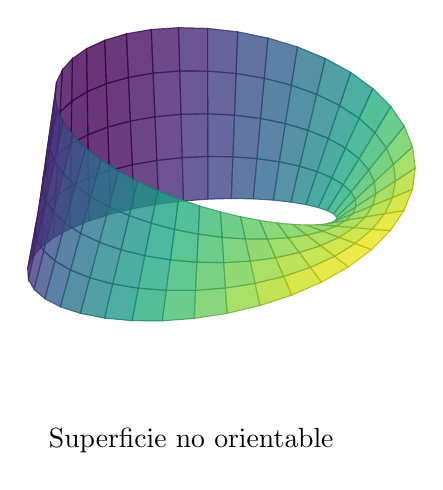
\begin{tikzpicture}
            \begin{axis}[
                hide axis,
                view = {40}{40},
                colormap/viridis,
            ]
                \addplot3 [
                    surf,
                    opacity=0.8,
                    point meta = x,
                    samples    = 40,
                    samples y  = 5,
                    z buffer   = sort,
                    domain     = 0:360,
                    y domain   = -0.5:0.5,
                ] (
                    {(1+0.5*y*cos(x/2)))*cos(x)},
                    {(1+0.5*y*cos(x/2)))*sin(x)},
                    {0.5*y*sin(x/2)}
                );
            \end{axis}
            \node[below] at (3,0) {Superficie no orientable};
        \end{tikzpicture}
    \end{minipage}
    \hfill
    % Second plot
    \begin{minipage}{0.48\textwidth}
        \centering
        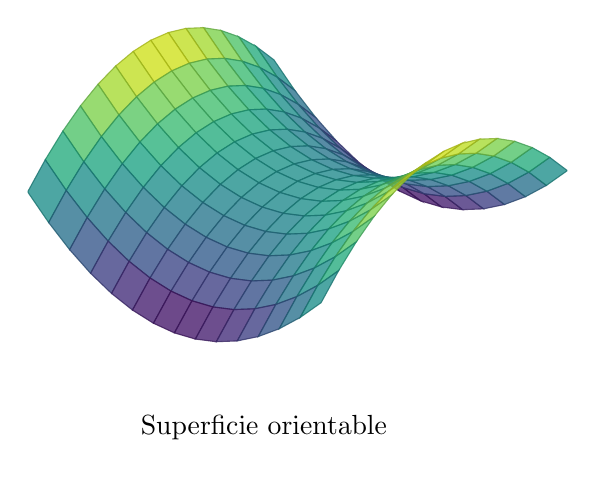
\begin{tikzpicture}
            \begin{axis}[
                hide axis,
                view={40}{40},
                colormap/viridis
            ]
                \addplot3[
                    surf,
                    opacity=0.8,
                    domain=-2:2,
                    samples=15
                ] {x^2 - y^2};
            \end{axis}
            \node[below] at (3,0) {Superficie orientable};
        \end{tikzpicture}
    \end{minipage}
\end{figure}


\end{example}

\begin{obs}
    Sea $S$ una superficie orientable. Entonces $S$ admite dos orientaciones posibles: $\boldsymbol{\eta}$ y $-\boldsymbol{\eta}$.
\end{obs}


 \textcolor{red}{Se podria explicar un poco más el ejemplo? }


\begin{definition}
    Sea $S\subseteq\Rn{3}$ una superficie orientada por $\boldsymbol{\eta}$. Sea $\boldsymbol{\Sigma}:D\subseteq\Rn{2}\to S$ una parametrizaci\'on continua de clase $\mathcal{C}^1$ y regular de $S$.
    \begin{itemize}
        \item Si \[
            \frac{\boldsymbol{\Sigma}_u\times\boldsymbol{\Sigma}_v}{\norm{\boldsymbol{\Sigma}_u\times\boldsymbol{\Sigma}_v}}(u,v)=\boldsymbol{\eta}\left(\boldsymbol{\Sigma}(u,v)\right),
        \]  
        decimos que $\boldsymbol{\Sigma}$ \textbf{preserva} la orientaci\'on de $S$.
        \item Si \[
            \frac{\boldsymbol{\Sigma}_u\times\boldsymbol{\Sigma}_v}{\norm{\boldsymbol{\Sigma}_u\times\boldsymbol{\Sigma}_v}}(u,v)=-\boldsymbol{\eta}\left(\boldsymbol{\Sigma}(u,v)\right),
        \]
        decimos que $\boldsymbol{\Sigma}$ \textbf{invierte} la orientaci\'on de $S$.  
    \end{itemize}
\end{definition}


 \textcolor{red}{OJO. Falta todo lo de campos escalares. }



\begin{definition}
    Sea $S\subseteq\Rn{3}$ una superficie orientada por $\boldsymbol{\eta}$. Sea $\mathbf{F}:A \subset \to\Rn{3}$ con $S\subset A$ un campo continuo. Se define la integral de superficie de $\mathbf{F}$ sobre $S$, y se nota  $\iint_S\mathbf{F}\cdot \mathbf{S},$ a
    \[
        \iint_S \mathbf{F}\;d\mathbf{S}=\iint_S (\mathbf{F}\cdot\boldsymbol{\eta}) \;dS.
    \]
\end{definition}

\begin{obs}   Sean $S\subseteq\Rn{3}$ una superficie orientada por $\boldsymbol{\eta}$ y  sea  $\boldsymbol{\Sigma}:D\subseteq\Rn{2}\to S\subseteq\Rn{3}$ una parametrizaci\'on de $S$ tal que preserve su orientaci\'on, entonces 

 $$ \iint_S \mathbf{F}\cdot d\mathbf{S} = \iint_D \mathbf{F}\circ\boldsymbol{\Sigma}\cdot\left(\boldsymbol{\Sigma}_u\times\boldsymbol{\Sigma}_v\right)dudv.$$
\end{obs}


Veamos que esto efectivamente es as\'i.  Sabemos que \textcolor{red}{por referencia}
\[
    \frac{\boldsymbol{\Sigma}_u\times\boldsymbol{\Sigma}_v}{\norm{\boldsymbol{\Sigma}_u\times\boldsymbol{\Sigma}_v}}(u,v)=\boldsymbol{\eta}\left(\boldsymbol{\Sigma}(u,v)\right).
\]
Entonces,
\begin{align*}
    \iint_S \mathbf{F}\cdot d\mathbf{S}&=\iint_S \mathbf{F}\cdot\boldsymbol{\eta}\;dS=\iint_D (\mathbf{F}\cdot\boldsymbol{\eta})\circ\boldsymbol{\Sigma}\:\norm{\boldsymbol{\Sigma}_u\times\boldsymbol{\Sigma}_v}\;dudv\\[.2cm]
    &=\iint_D (\mathbf{F}\circ\boldsymbol{\Sigma})\cdot(\boldsymbol{\eta}\circ\boldsymbol{\Sigma})\norm{\boldsymbol{\Sigma}_u\times\boldsymbol{\Sigma}_v}\;dudv=\iint_D \mathbf{F}\circ\boldsymbol{\Sigma}\cdot\left(\boldsymbol{\Sigma}_u\times\boldsymbol{\Sigma}_v\right)dudv,
\end{align*} concluyendo lo que quer\'iamos ver.

\begin{obs}
    Sea $S$ una superficie con orientaci\'on $\boldsymbol{\eta}$. Sea $\boldsymbol{\Sigma}:D\subseteq\Rn{2}\to S\subseteq\Rn{3}$, una parametrizaci\'on de $S$ que invierte la orientaci\'on. Entonces
    \[
        \iint_S \mathbf{F}\cdot d\mathbf{S} = \iint_S \mathbf{F}\cdot\eta\;dS=-\iint_D \mathbf{F}\circ\boldsymbol{\Sigma}\cdot(\boldsymbol{\Sigma}_u\times\boldsymbol{\Sigma}_v)\:dudv.
    \]
\end{obs}

